\chapter{Use Case 1: WorldData Explorer}

\section{Einführung}
Im ersten Use Case geht es hauptsächlich um die Anzeige grosser Datenmengen auf der Karte. Dazu importieren wir bestehende Datenbestände in die Google Fusion Tables und visualisieren diese mittels Google Maps API auf der Karte.

\subsection{Ziel}
Es sollen verschiedene historische Länderdaten auf einer Weltkarte angezeigt werden. Die Daten sind pro Jahr und Thema unterteilt. Über eine Zeitachse soll es möglich sein die Daten der verschiedenen Jahre zu selektieren. Eine solche Darstellung kann beispielsweise dabei helfen Zusammenhänge zwischen verschiedenen Themenbereichen zu finden.

\subsection{Vorgehen}
Um die Daten pro Land zu visualisieren, werden zuerst die Landesgrenzen als Geometrie-Datensätze in eine separate Fusion Tabelle importiert. In eine andere Tabelle werden dann die Daten importiert unterteilt nach Land und Jahr. Diese beiden Tabellen werden per Merge-Funktion zu einer Tabelle zusammengefasst, welche dann mittels FusionTablesLayer auf der Karte dargestellt werden kann.

\subsubsection{ERD}
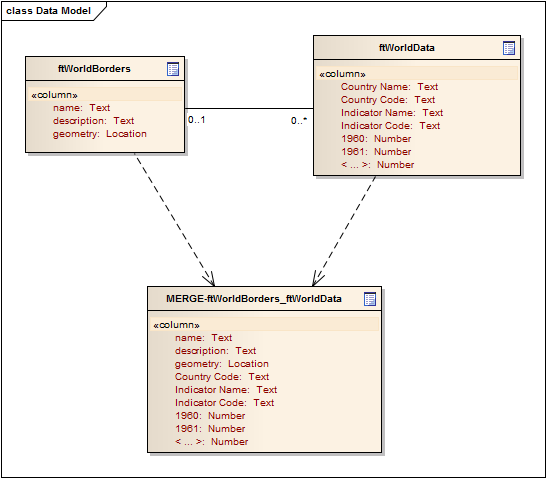
\includegraphics[scale=0.8]{images/usecase1-worlddata-erd.png}

\subsection{Datenquellen}
Als Datenquelle wurde der Daten Katalog der Weltbank (\url{http://data.worldbank.org/}) verwendet. Darin finden sich länderspezifische Daten aufgeteilt in über 7000 Themenbereiche.

Die Landesgrenzen wurden als \gls{KML}-Datei von einer inoffiziellen Google Earth Library-Webseite (\url{http://www.gelib.com/world-borders.htm}) bezogen. 

\section{Anforderungsspezifikation}

\section{Analyse}

\section{Design}

\section{Implementation}

\section{Test}

\section{Resultate}

\section{Weiterentwicklung}

\section{Benutzerdokumentation}